%%%%%%%%%%%%%%%%%%%%%%%%%%%%%%%%%%%%%%%%%
% Thin Sectioned Essay
% LaTeX Template
% Version 1.0 (3/8/13)
%
% This template has been downloaded from:
% http://www.LaTeXTemplates.com
%
% Original Author:
% Nicolas Diaz (nsdiaz@uc.cl) with extensive modifications by:
% Vel (vel@latextemplates.com)
%
% License:
% CC BY-NC-SA 3.0 (http://creativecommons.org/licenses/by-nc-sa/3.0/)
%
%%%%%%%%%%%%%%%%%%%%%%%%%%%%%%%%%%%%%%%%%

%----------------------------------------------------------------------------------------
%	PACKAGES AND OTHER DOCUMENT CONFIGURATIONS
%----------------------------------------------------------------------------------------

\documentclass[11pt]{article} % Font size (can be 10pt, 11pt or 12pt) and paper size (remove a4paper for US letter paper)

\usepackage[utf8]{inputenc} % Set utf8 code
\usepackage[protrusion=true,expansion=true]{microtype} % Better typography
\usepackage[portuguese]{babel}
\usepackage{graphicx} % Required for including pictures
\usepackage{wrapfig} % Allows in-line images
\usepackage{hyperref}

\usepackage{mathpazo} % Use the Palatino font
\usepackage[T1]{fontenc} % Required for accented characters
\linespread{1.05} % Change line spacing here, Palatino benefits from a slight increase by default

\makeatletter
\renewcommand\@biblabel[1]{\textbf{#1.}} % Change the square brackets for each bibliography item from '[1]' to '1.'
\renewcommand{\@listI}{\itemsep=0pt} % Reduce the space between items in the itemize and enumerate environments and the bibliography

\renewcommand{\maketitle}{ % Customize the title - do not edit title and author name here, see the TITLE block below
\begin{center} % Right align
{\LARGE\@title} % Increase the font size of the title

\vspace{20pt} % Some vertical space between the title and author name

\end{center}
}

\begin{document}

\begin{titlepage}
 \vfill
  \begin{center}
   {\large \textbf{Tiamat}} \\
   {\large \textbf{Babel}}\\[6cm]


   {\Large Documento de visão}\\[6cm]

   \hspace{.45\textwidth} %posiciona a minipage
  \vfill

\vspace{2cm}

\large \textbf{Brasília}

\large \textbf{Abril de 2015}
\end{center}
\end{titlepage}
\newpage
%----------------------------------------------------------------------------------------
%	DOC BODY
%----------------------------------------------------------------------------------------

\section*{Apresentação}

Babel é um jogo \textit{Sci-Fi} do tipo \textit{Dungeon Crawler's} RPG com mecânicas de manejamento de recursos.

\section*{Resumo}

\paragraph{}A Terra está morta, após milhares de anos de ganância, a raça humana conseguiu exaurir os recursos do planeta.  Indignados com o destino que eles mesmo fizeram para eles, a raça humana se prepara para uma última jornada, à procura de um planeta que possam chamar de seu. Um  último suspiro antes de mergulhar na vastidão do espaço.

\paragraph{}Após anos vagando no espaço, em seus sonhos congelados, os mais sensíveis começaram a ter estranhos sonhos, quase visões. Caso estes não estivessem dormindo, seriam estes visões de um planeta, um novo mundo de esperança.

\begin{figure}[!htp]
\centering
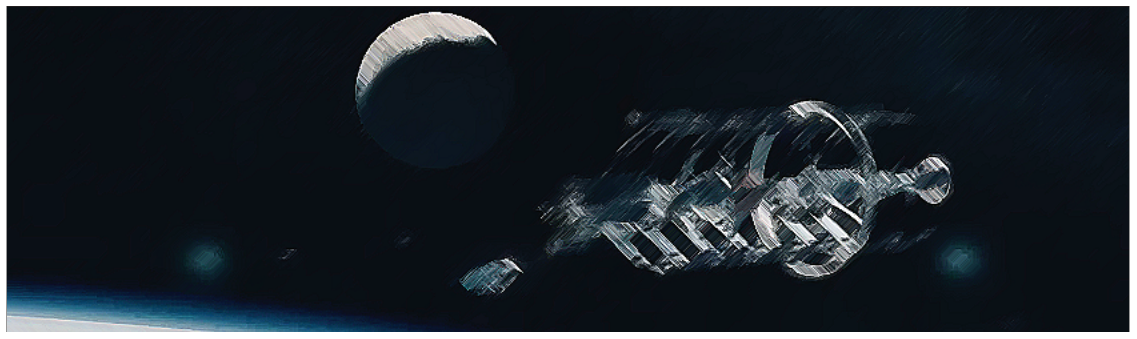
\includegraphics[scale=0.3]{res/history.png}
\caption{Nave Espacial}
\label{Nave Espacial}
\end{figure}

\paragraph{}E dentro daquela espora espacial, um pequeno som ecoou dentro dos corredores apertados. Um sinal, vindo do que poderia ser apenas o impossível. Uma imensa torre se projetava da superfície de um planeta próximo. A torre, assim como o planeta, não mostrava nenhum sinal de vida.

\newpage

\begin{figure}[!htp]
\centering

\includegraphics[scale=0.4]{res/tower.png}
\caption{Torre}
\label{Torre}
\end{figure}

\paragraph{}Mal esperavam abrir os olhos, os tripulantes já falavam da Torre, na verdade, quase que exclusivamente dela. Pousaram no planeta, decisão unânime, definitivamente, um sinal. De quem? Aliens? Deus? Estas perguntas foram soltas juntas com o último sistema de propulsão da nave, enquanto esta se preparava para concretizar o último desejo humano, o desejo de sobreviver.

\section*{Principais características}

\paragraph{}Uma das características que fazem o jogo ser diferenciado em relação aos demais \textit{Dungeon Crawler's} é o fato de este possuir explorações tanto horizontais e verticais. 

\newpage

\begin{figure}[!htp]
\centering

\includegraphics[scale=0.3]{res/mechanics.png}
\caption{Mecânicas}
\label{Mecânicas}
\end{figure}

\paragraph{}Na exploração horizontal o jogador deverá explorar o novo planeta a fim de encontrar recurso para que este possa evoluir seus itens disponíveis. 

\begin{figure}[!htp]
\centering
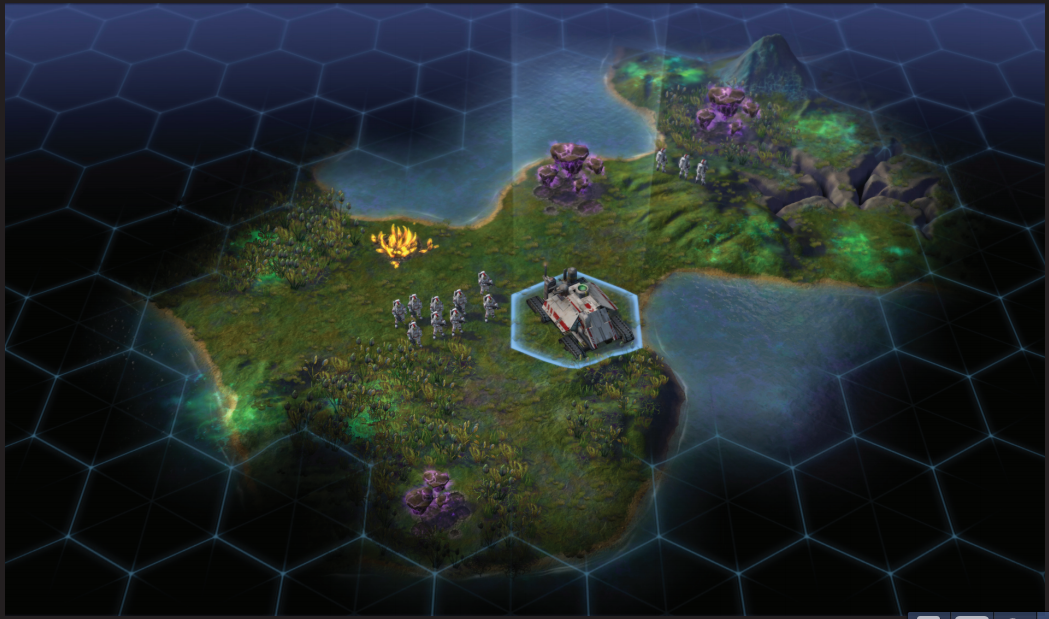
\includegraphics[scale=0.3]{res/resources.png}
\caption{Exploração Horizontal}
\label{Exploração Horizontal}
\end{figure}

\paragraph{}No sentido vertical, o jogador irá explorar a torre com os objetivos de desvendar novas tecnologias dentro da torre para aumentar a chance de sobrevivência e de descobrir que tipo de ser seria capaz de construir tal monumento e quais impactos esse ser poderia causar a raça humana.

\newpage

\begin{figure}[!htp]
\centering
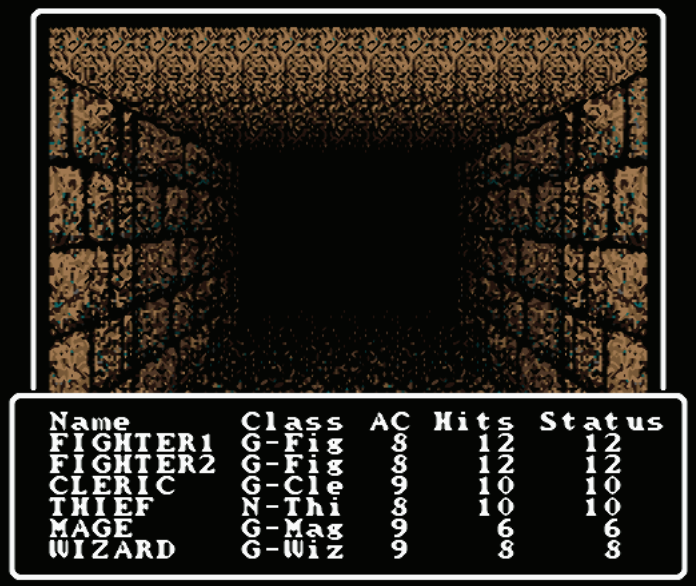
\includegraphics[scale=0.3]{res/Dungeon_Crawler.png}
\caption{Exploração Vertical}
\label{Dungeon Crawler}
\end{figure}

\section*{Público Alvo}

\paragraph{}O público alvo será para os maiores de 12 anos. O jogo conterá atos violentos, presença de sangue, exposição de cadáveres, etc.

\section*{Plataformas Alvo}
\begin{itemize}
\item \textbf{Linux:} O Linux será uma plataforma alvo, pois será neste ambiente onde o jogo deverá ser desenvolvido e por esse sistema operacional possuir um número relativamente baixo de jogos comparado ao Windows aumentando assim as chances de atingirem os seus usuários. 

\item \textbf{Windows:} O Windows será uma plataforma alvo pelo simples fato de este sistema operacional possuir um enorme número de usuários jogadores.
\end{itemize}

\section*{Esquema de controle e interface com o usuário}
Com relação a exploração vertical, dentro da torre, esta será em primeira pessoa, sendo que serão utilizadas as teclas destacadas na figura a seguir:\\
\begin{figure}[!htp]
\centering
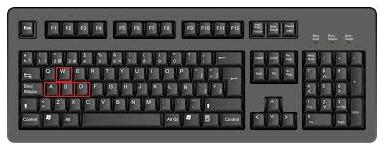
\includegraphics[scale=0.75]{res/keyboard.jpg}
\caption{Teclas utilizadas}
\label{Teclado}
\end{figure}
\\Onde a tecla ''w'' irá movimentar o jogador para frente, a tecla ''s'' irá movimentar o jogador para trás, a tecla ''a'' irá rotacionar o jogador $90\,^{\circ}$ para a esquerda e a tecla ''d'' irá rotacionar o jogador $90\,^{\circ}$ para a direita.

Com relação a exploração horizontal, na superfície do mundo, o jogador irá usar o \textit{mouse} para navegar na superfície, utilizando o botão direito para selecionar algum objeto e o botão esquerdo para movimentar algum objeto, atacar inimigos e coletar recursos. 
\section*{Descrição dos recursos tecnológicos notáveis}

\begin{itemize}
\item \textbf{Cubase}: Ferramenta avançada utilizada para criar músicas, com ela é possível compor, gravar, editar e mixar áudio e arquivos MIDI. Essa ferramenta suporta surround 5.1

\begin{figure}[!htp]
\centering

\includegraphics[scale=0.3]{res/cubase-Logo.png}
\caption{Logo do Cubase}
\label{Cubase}
\end{figure}

\item \textbf{Audacity}: Ferramenta livre que possibilita a importação, exportação, edição e gravação de diversos formatos de áudio.

\begin{figure}[!htp]
\centering

\includegraphics[scale=0.3]{res/audacity.jpg}
\caption{Logo do Audacity}
\label{Audacity}
\end{figure}

\item \textbf{Adobe Illustrator}: Ferramenta para ilustração gráfica e criação vetorial.

\begin{figure}[!htp]
\centering

\includegraphics[scale=0.3]{res/adobe_illustrator.png}
\caption{Logo do Adobe Illustrator}
\label{Adobe Illustrator}
\end{figure}

\item \textbf{Adobe Photoshop}: Ferramenta profissional de edição de imagens, com ela é possível fazer recortes de elementos, aplicar filtros e máscaras, etc.

\begin{figure}[!htp]
\centering

\includegraphics[scale=0.3]{res/Photoshop.png}
\caption{Logo do Adobe Photoshop}
\label{Adobe Photoshop}
\end{figure}

\item \textbf{SDL2}: É uma biblioteca livre multiplataforma para desenvolvimento de jogos e aplicações multimídia.

\begin{figure}[!htp]
\centering

\includegraphics[scale=0.3]{res/Sdl-logo.png}
\caption{Logo do SDL2}
\label{SDL2}
\end{figure}

\item \textbf{Sublime text}: Editor de texto desenvolvido em C++.

\begin{figure}[!htp]
\centering

\includegraphics[scale=0.3]{res/Sublime_Text_Logo.png}
\caption{Logo do Sublime text}
\label{Sublime text}
\end{figure}

\end{itemize}

\section*{Informações de contato}
A equipe \textbf{Tiamat} pode ser contatada pelo seguinte endereço de e-mail: \href{mailto:tiamatbabel@gmail.com}{tiamatbabel@gmail.com}.

Caso o contato seja para contribuir com o jogo e/ou relatar algum \textit{bug} basta acessar o repositório o oficial do \textbf{Babel} no seguinte endereço: \url{https://github.com/ije-tiamat/babel}.

\end{document}
